\section{Unordered Delivery in MPEG-DASH}
\label{sec:transport}

MPEG-DASH is designed for an ordered transport protocol. Adapting it for an
unordered transport protocol requires several considerations. These
changes happen in two broad areas: the HTTP request and response semantics, and the rate
adaptation algorithms. We consider both of these in turn below.

\subsection{HTTP Request/Response Semantics}

TCP Hollywood operates on a message level and thus the decision to keep or discard is made
for a message. The application must therefore decide what each message should contain. In
the case of our HAS application, messages could contain either (i) an entire chunk of video; 
(ii) a video frame from within the chunk; or (iii) a fixed-sized message from within the 
chunk boundaries.  Sending an entire chunk as a TCP Hollywood
message means that the loss of a single TCP segment carrying part of that message could result in
the entire message being lost if it failed to be delivered before its deadline. Sending 
individual video frames would require the HTTP server to be content-aware, and able to 
split video chunks into frame; this is beyond the scope of our work given our goal of
maintaining alignment with the MPEG-DASH standard. Accordingly, we opt to send fixed-size 
messages (of 1400 bytes), which balances the impact of segment loss with being content-agnostic. 
The terminology and its use within the paper is further clarified in Figure \ref{fig:terminology}.

\begin{figure}
  \centering
  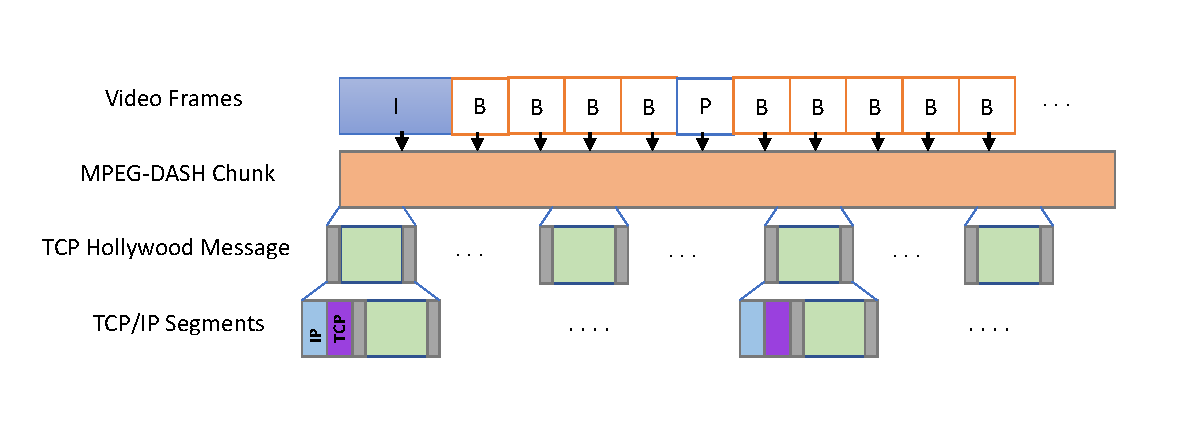
\includegraphics[width=\columnwidth]{figures/terminology2.pdf}
  \caption{Illustration of the terminology used in this paper and also the encapsulation of data for transport.}
  \label{fig:terminology}
\end{figure}

TCP Hollywood supports multi-streaming over a single TCP connection, allowing for the
separation of the control and data channels. We use separate streams for HTTP request and
response headers, sending each as separate TCP Hollywood messages. This allows the client
to request later chunks while earlier chunks are still downloading. The server still sends
chunks sequentially, but does not have to wait for the next request to arrive; this is
especially useful in high latency networks. Figure \ref{fig:hollywood_download}
illustrates chunk retrieval with HTTP over both standard TCP and TCP Hollywood.

Our use of multi-streaming in TCP Hollywood is similar to HTTP/1.1 pipelining and bundle
requests in HLS \cite{muller2012evaluation}. However, these approaches require quality
estimates to be submitted for all chunks at request time. This means that a quality
estimate may be two or more chunk durations old before being used at the server.
Fluctuations in network conditions in the interval between request and response mean that
these quality estimates can be incorrect. Under TCP Hollywood, requests can be sent while
chunks are downloading, allowing for the server to receive a more recent and accurate
estimate of network conditions. This reduces the likelihood of an under or over estimation
of performance, improving quality-of-experience. Further, HTTP/1.1 pipelining suffers
from transport-layer head-of-line blocking in standard TCP, which is eliminated under TCP Hollywood.

Finally, TCP Hollywood can discard late messages and continue play-out,
thereby limiting stall events only to those cases when the play-out buffer is completely
empty.

\begin{figure}
    \centering
    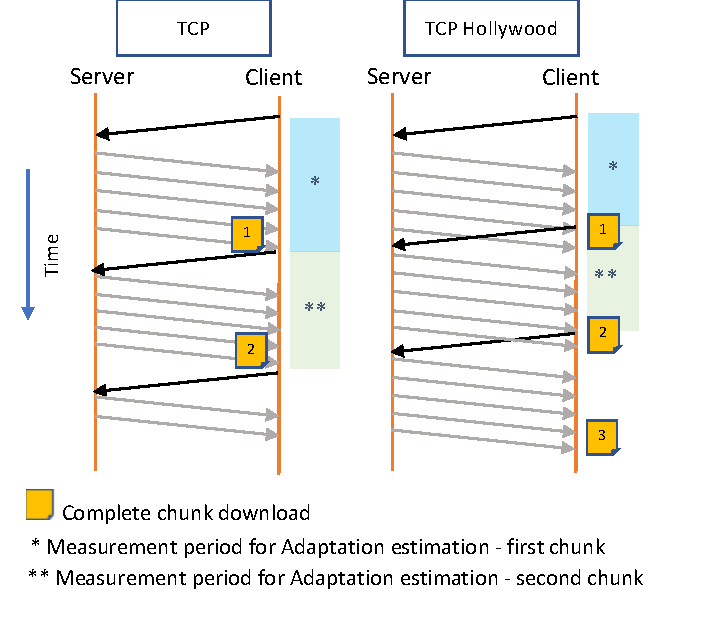
\includegraphics[width=\columnwidth]{figures/tcph-download.pdf}
    \caption{An illustration of chunk download with HTTP over TCP and over TCP Hollywood}
    \label{fig:hollywood_download}
    % FIXME: what are the light blue and light green shaded rectangles in this figure? [csp]
\end{figure}

The requested chunks of video are transmitted on a single stream, using fixed size
messages. As the server is content-agnostic, it is unable to set an expiry time for messages, and
all messages are sent reliably. A content-aware server would set this to the relative presentation time of the chunk.
For the sake of simplicity, audio
stream is not used. Each message is appended with a monotonically increasing sequence
number and a stream offset. The stream offset is the offset of the last byte of the
message within this stream, where a stream includes all chunks that have been transmitted
previously. Both fields are used by the receiver to reorder the messages and detect
losses. We expanded the function of the play-out buffer to include de-jittering and
reordering of the incoming messages.

% FIXME: explain why MP4 is not suitable [csp]
It is also important to use a media format that is tolerant of packet losses. Hence, the
commonly used ISO Base Media File Format (MP4) is not suitable for TCP Hollywood, so we
use MPEG Transport streams (TS) instead. The use of MPEG-TS streams is allowed as part of
the MPEG-DASH standard and are also used by HLS.

\subsection{Rate Adaptation Algorithms}

Performance of a MPEG-DASH system relies heavily on a good rate adaptation algorithm.
Such algorithms use application-level measurements such as buffer length, throughput, time to
download a chunk, or a combination of these to select an appropriate quality for
download \cite{beben2016abma+, spiteri2016bola, li2014probe}. There is some consensus
among researchers that buffer-based algorithms are more performant and reliable in a wider
variety of network conditions than other algorithms 
\cite{huang2015buffer, karagkioules2017comparative}.

Our TCP Hollywood-based MPEG-DASH client uses a modified version of the open-source BOLA 
(Buffer Occupancy based Lyapunov Algorithm) rate adaptation algorithm \cite{spiteri2016bola}. 
BOLA is part of the MPEG-DASH reference
client, dash.js.\footnote{\url{https://github.com/Dash-Industry-Forum/dash.js/wiki}}
BOLA uses the amount of video currently buffered to calculate the quality level (bit-rate
level) for the next chunk. For live video, where buffer sizes are limited, the algorithm
uses throughput estimates to further reduce over-estimation and stalling. In the presence
of packet loss and duplication, that is possible with TCP Hollywood, the calculation 
mechanisms for both measurements have to be modified. For a standard MPEG-DASH client,
the HTTP request for the next chunk is always sent 
during the download of the current chunk. For our TCP Hollywood-based client, we
introduce a new parameter, $Rx_{T}$, the receive ratio threshold. We modify
the rate adaptation algorithm so that if $Rx_{T}$ of the
bytes from a chunk have been received and the buffer is not filled to capacity, 
it estimates the quality of the next chunk based on the \emph{current} measurements and
sends a GET request to the server. Throughput is measured from the time the HTTP response
of a chunk arrives until $Rx_{T}$ is reached, excluding any duplicates. We experimented
with different values of $Rx_{T}$ and found 0.9 to be a suitable ratio. The full duration
of the chunk is used when calculating the buffer level, even though the entire chunk has
not been downloaded. With an $Rx_{T}$ value of 0.9, this is a safe assumption: only 10\%
of the chunk remains to be downloaded, with some data in-flight, and a limited number of
messages that may delayed (and subsequently discarded by TCP Hollywood if
they miss their deadline).
% FIXME: probably outside the scope of the initial submission, but it would
% be appropriate to describe the experiments and results that led to the
% choice of 0.9 as a parameter [csp]

% FIXME: "uses an effective buffer level" to do what? [csp]
BOLA uses an effective buffer level in the event that the chunk download is slowed by
the availability of the next chunk at the server (e.g., it has not been captured yet, as
in live scenarios) or by the size of the play-out buffer. In this case, as the buffer level has not
been limited by network conditions, the client is able to request higher quality chunks.
Therefore, the effective buffer level is the current buffer level, plus the time spent
waiting before downloading the next chunk. With TCP Hollywood, messages may be discarded
due to late arrival. If the buffer contains more than one chunk, we reduce the length of
effective buffer level by one chunk duration.

%
%For the latter, we use the parameter rxratio (Receive ratio); the receiver will stop
%actively receiving a chunk if it has already received rxratio times the total bytes in
%the chunk and move on to estimating quality and requesting the next chunk. Since we use a
%buffer based algorithm, we still assume that we have received the entire chunk while
%calculating the quality of the next chunk. Note that the remaining chunk is still being
%received passively, which means that the data is not used in throughput calculations for
%the adaptation algorithm. 
%
